\documentclass[12pt]{article}
\usepackage{amsmath,epsfig, subfigure, multirow}
\usepackage{multirow}
\usepackage{geometry}
%\geometry{a4paper}
\geometry{left=18mm,right=18mm,top=21mm,bottom=21mm}

%\gemoetry{verbose,a4paper,tmargin=21mm,bmargin=21mm,lmargin=18mm,rmargin=18mm}
\usepackage{graphics}
\usepackage{setspace}
\newcommand{\Lyx}{L\kern-.1667em\lower.25em\hbox{y}\kern-.125emX\spacefactor1000}
\newcommand\bibname{References}
\singlespacing
\begin{document}
\bibliographystyle{ieeetr}
\pagestyle{plain} 
\pagenumbering{arabic}
%\rmfamily

\title{Modeling the Quantization Staircase Function}
\author{
Salman Aslam, Aaron Bobick, Christopher Barnes\\   
Georgia Institute of Technology,\\
Atlanta, 30332,\\
USA
}
%\date{31 May, 2002}
\maketitle

% Article starts here

%---------------------------------------------------------------------------------------------------------------------------------
%ABSTRACT
%---------------------------------------------------------------------------------------------------------------------------------
\begin{abstract}
Quantization plays a central role in data compression.  In speech systems, vector quantizers are used to compress speech parameters.  In video systems, scalar quantizers are used to reduce variability in transform coefficients.  More generally, quantizers are used to compress all forms of data.  In most cases, the quantizers are based on some form of staircase function.  Deriving an analytical expression for a uniform midrise quantizer is well known and straightforward.  In this paper, we create an alternate method of deriving such an analytical expression with the hope that the steps involved will be useful in understanding quantization and its various applications.  
\end{abstract}

{\bf Keywords:} Quantization, Compression, Uniform quantizer, Midrise quantizer.\\

%------------------------------------------------------------------------------------------------------------------------------
\section{INTRODUCTION}
%------------------------------------------------------------------------------------------------------------------------------
Our goal is to model the quantization staircase function as given in Figure~\ref{fig:Staircase}.  This is a shifted $uniform \ midrise \ quantizer$~\cite{2005_BOOK_DataCompression_Sayood}.  For our purposes, the shift does not lead to any loss in generality.  Writing an equation for this quantizer is well-known and relatively straightforward, and is given as $Model 1$ below.  In this paper, our goal is to present $Model 2$, an alternate form of modeling the quantization function in the hope that such a model could be helpful in designing quantizers~\cite{1982_JNL_LeastSquaresQuantization_Lloyd}~\cite{1991_BOOK_VQ_GershoGray}~\cite{1996_JNL_AdvancesRVQ_Barnes}~\cite{1997_BOOK_SignalCompression_Jayant}, modeling source-channel distortion~\cite{2009_JNL_MPEG4JointSourceChannelDistortion_Sabir}, video traffic modeling~\cite{2002_JNL_MPEG2traffic_Ansari}, RDO estimation~\cite{2007_JNL_H264rateDistortion_Yang}, rate-quantization modeling~\cite{1996_JNL_MPEG4RateControl_Wei} and preserving semantic information in compressive channels~\cite{2009_CNF_CVcompMS1_Aslam}~\cite{2009_CNF_Compensation_Aslam}~\cite{2009_CNF_RobustSurveillance_Aslam}.  Our method is based on the Continuous Time Fourier Series (CTFS).

		%figure: staircase
		\begin{figure}[t]
		\centering
		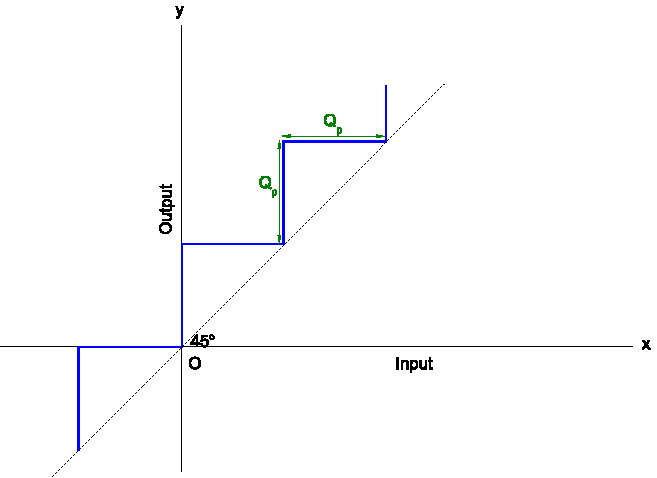
\includegraphics[width=0.45\textwidth]{figs/Quantization_1_staircase}
		\caption{A staircase function, (shifted $uniform \ midrise \ quantizer$).}
		\label{fig:Staircase}
		\end{figure}

%------------------------------------------------------------------------------------------------------------------------------
\section{THEORY}
%------------------------------------------------------------------------------------------------------------------------------
		
		%figure: Model1
		\begin{figure}[t]
		\centering
		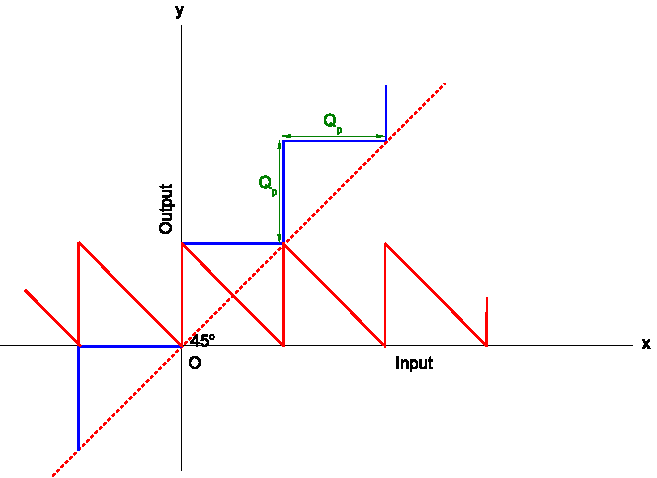
\includegraphics[width=0.45\textwidth]{figs/Quantization_2_staircase_residual}
		\caption{Model 1.  Creating a staircase function by adding the input to a sawtooth wave.}
		\label{fig:Model1}
		\end{figure}

		%figure: Model2
		\begin{figure}[t]
		\centering			
		\subfigure[Integrating a square wave with $50\%$ duty cycle to yield a right angled isosceles triangle.]
		{
			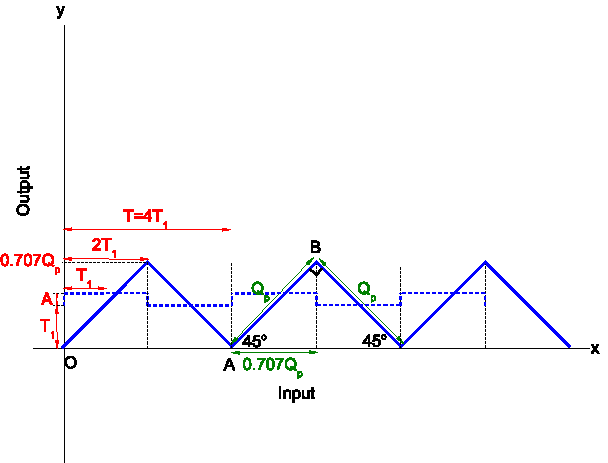
\includegraphics[width=0.45\textwidth]{figs/Quantization_3_triangle_wave}
			\label{fig:Model2_a}
		}			
		\subfigure[Working with the rotated triangle wave.]
		{
			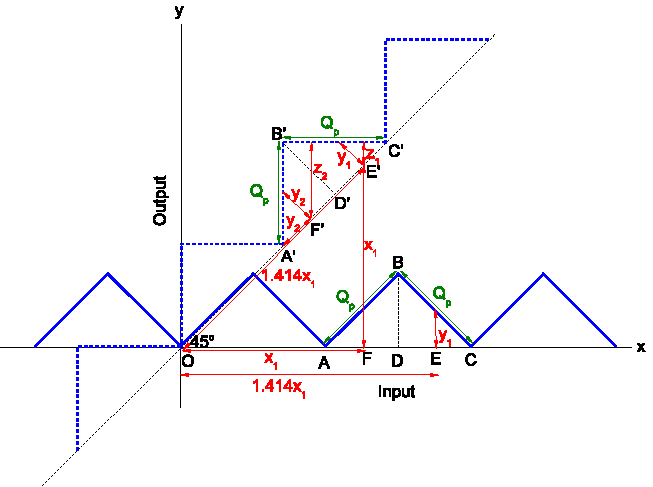
\includegraphics[width=0.45\textwidth]{figs/Quantization_4_rotated_triangle_wave}
			\label{fig:Model2_b}
		}
		\subfigure[Working with the unrotated triangle wave.]
		{
			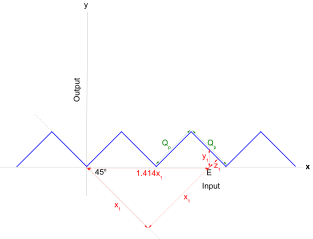
\includegraphics[width=0.45\textwidth]{figs/Quantization_5_triangle_wave}
			\label{fig:Model2_c}					
		}
		\caption{Model 2.  Creating a staircase function by adding the input to a sawtooth wave.  Here, the sawtooth wave is computed using a succession of CTFS.}
		\label{fig:Model2} 						
		\end{figure}
					
\subsection{Continuous Time Fourier Series}
%--------------------------------------------------
The CTFS produces a discrete representation of a continuous time periodic signal.  The analysis equation of the complex representation of the series is given by,

		\begin{equation}
		c[k]=\frac{1}{2\pi} \int_{\frac{-T}{2}}^{\frac{T}{2}} f(t)e^{-jkw_0t}dt\\
		\label{eq:Fourier_Series_Analysis}
		\end{equation}
	
where $f(t)$ is the signal under study with time period $T$, and $w$ is the radian frequency.  The output coefficients $c[k]$ represent the amplitudes of the spectrum of $f(t)$ at discrete frequencies $w_k$.  The CTFS is an invertible transformation and the corresponding synthesis equation is given by,

		\begin{equation}
		f^{'}(t)= \sum_{k=-\infty}^{k=\infty} c[k]e^{jkw_{0}t}\\
		\label{eq:Fourier_Series_Synthesis}
		\end{equation}		
 						 	 	
		   				
\textbf{Square Wave.}  For a standard, non-negative square wave centered around the Y-axis, having period $T$ and amplitude $A$ from $-T_1$ to $T_1$, i.e. on for a time duration of $2T_1$ and 0 otherwise during a single time period $T$, the CTFS coefficients are

		\begin{equation}
		c[k] = \frac{2 A sin(kw_0T_1)}{(kw_0T)}
		\label{eq:Square_Wave_standard}
		\end{equation}
				
This is a standard sinc function.  $w_0T = 2\pi$ but we write it in the form above to introduce some degree of symmetry.  Using L'Hopital's Rule, $c[0]= 2A\frac{T_1}{T}$.  We can introduce some variations in this square wave.  First, if we set $c[0]=0$, we get a square wave that is symmetric around the X axis.  Second, we can introduce a time shift $t_0$, and a DC shift $y_0$, in this square wave, as follows,

		\begin{align}
		c[k] &= \frac{2 A sin(kw_0T_1)}{(kw_0T)}e^{-jkw_0t_0}, k\neq 0\notag\\
		c[0] &= y_0 + \frac{2AT_1}{T}, k=0 
		\label{eq:Square_Wave_shifted}
		\end{align}	

\textbf{Triangle Wave.}  We can also integrate this square wave in the time domain to create a triangle wave.  In the frequency domain, this amounts to dividing by $jkw_0$,

		\begin{equation}
		c[k] = \frac{\frac{2 A sin(kw_0T_1)}{(kw_0T)}}{jkw_0}e^{-jkw_0t_0}
		\label{eq:Shifted_Triangle_Wave}
		\end{equation}	
						
This triangle wave stretches between the following negative and positive amplitudes,

		\begin{align}
 		Negative \ amplitude &= -AT_1 + \frac{2AT_1^2}{T}\notag\\
 		Positive \ amplitude &= AT_1 - \frac{2AT_1^2}{T}
 		\label{eq:Triangle_Wave_Amplitudes}
 		\end{align}
 		
%------------------------------------------------------------------------------------------------------------------------------
\section{DETAILS: Model 1}
%------------------------------------------------------------------------------------------------------------------------------
		%figure: Linear in Qq
		\begin{figure}[t]
		\centering				
		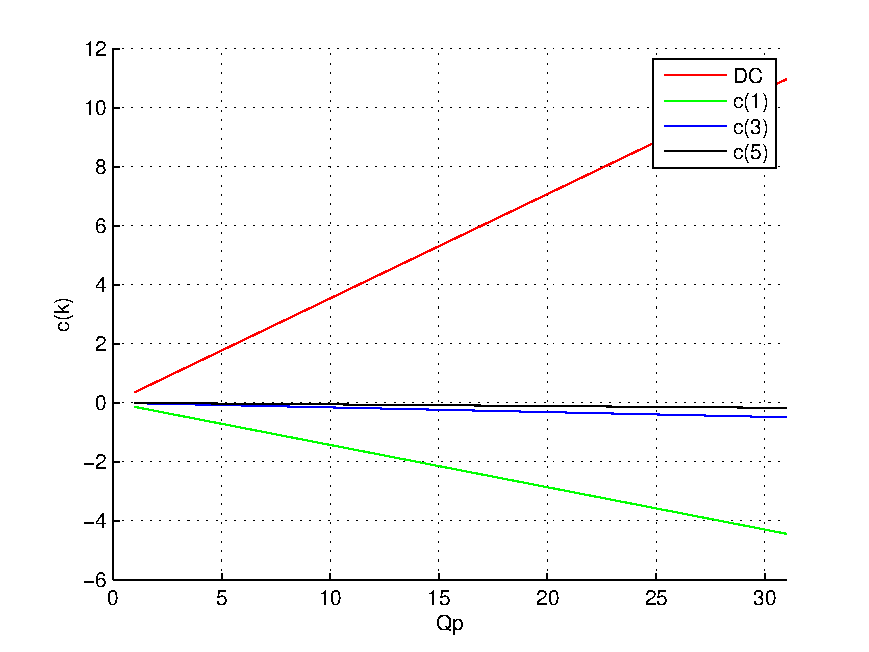
\includegraphics[width=0.45\textwidth]{figs/Quantization_6_first_triangle_wave_coefficients_linear_in_Qp}
		\caption{Coefficients of the triangle wave generated in the first step are linear in $Qp$.}
		\label{fig:Linear_in_Qp}
		\end{figure}
		
The first method, called $Model 1$,  is to model the staircase as the input added to a residual sawtooth wave (Figure~\ref{fig:Model1}).  A sawtooth wave can be generated using Equation~\ref{eq:Shifted_Triangle_Wave}.  For instance, a sawtooth wave that stretches between amplitudes $\pm5$ can be generated using $T=10$, $T_1=0.1$, and $A=51.02$. The resulting staircase function is plotted in Figure~\ref{fig:Matlab_StaircaseFunction_Models_1_2}.  

%------------------------------------------------------------------------------------------------------------------------------
\section{DETAILS: Model 2}
%------------------------------------------------------------------------------------------------------------------------------

The second method, called $Model 2$ is based on the following steps:
  
\begin{itemize}
\item \textbf{Square wave 1}.  We start with the square wave in Equation~\ref{eq:Square_Wave_shifted}, and using parameters, %$A=2, T1=\frac{Qp}{\sqrt{8}}, T=4T_1= \sqrt{2}Qp, w_0=\frac{2\pi}{T} = \frac{\sqrt{2}\pi}{Qp}, %t_0=T_1, y_0=T_1$, 

		\begin{align}
		\label{eq:Parameter_values_1}
		A		&=	2\notag\\
		T1	&=	\frac{Qp}{\sqrt{8}}\notag\\ 
		T		&=	4T_1\notag\\
		w_0	&=	\frac{\sqrt{2} \  \pi}{Qp}\notag\\ 
		t_0	&=	T_1\\
		y_0	&=	T_1\notag
		\end{align}	
		
we get,
	
		\begin{equation}
		c_{s_1}[k] = \frac{sin(a)}{a}e^{-ja}
		\label{eq:Square_1_ck}
		\end{equation}
		
where $a=k\pi/2$.  We use the subscript $s_1$ to denote that this is the first square wave we are using.  Notice that the forward dependence of $T_1$, and the inverse dependence of $w_0$ and $t_0$ on $Qp$ means that $c_{s_1}[k]$ does not depend on it.  Also, $c[0]$ and all even coefficients are $0$.  Odd coefficients are imaginary.  $c_{s_1}[k]$ is an odd function, i.e.  $-c_{s_1}[-k]$ = $c_{s_1}[k]$.

 		%approximations
		\begin{figure}
		\centering
		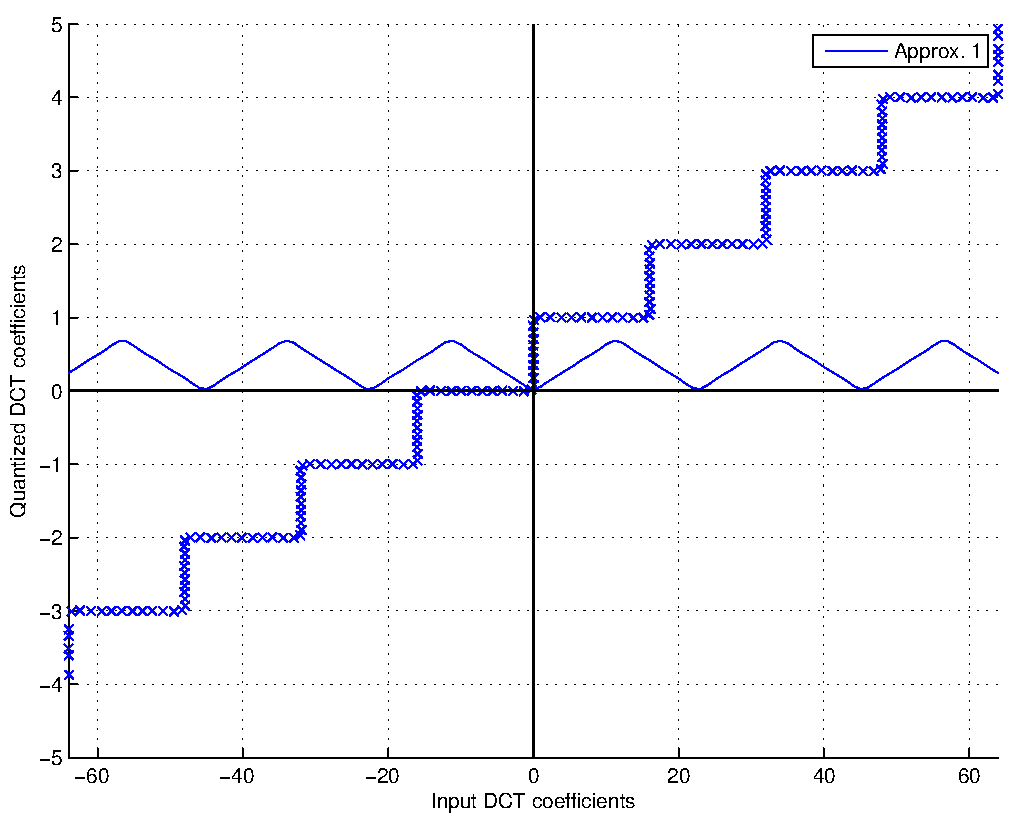
\includegraphics[width=.45\textwidth]{figs/Quantization_7_result_plot_first_triangleWave}		
		\caption{Approximations of staircase function using rotated triangle waves.}
		\label{fig:Creating_model_2} 		
    \end{figure} 
    
\item \textbf{Triangle wave}.  We integrate the square wave above to generate a triangle wave, as shown in Equation~\ref{eq:Shifted_Triangle_Wave}.  The parameters for the square wave were chosen to get a right angled isosceles triangle with base and perpendicular equal to $Qp$, as shown in Figure~\ref{fig:Model2_a}.  We see that division by the term $jkw_0$ introduces a linear dependence on $Qp$ as shown in Figure~\ref{fig:Linear_in_Qp} and given below,

		\begin{align}
		c_t[k] &= \frac{c_{s_1}[k]}{jkw_0}\notag\\
		       & =  \frac{Qp}{j \sqrt{2} \ \pi \ k}  \ c_{s_1}[k]
		\label{eq:Triangle_1_ck}
		\end{align}
		
$c[0]$ and the even coefficients are again all $0$.  Odd coefficients are real.  $c_{t}[k]$ is an even function. i.e. $c_{t}[-k]$ = $c_{t}[k]$.  $c_{t}[1]= \ 0.1433 \ Qp, c_{t}[3]= \ 0.0159 \ Qp, c_{t}[5]= \ 0.0057 \ Qp$ and so on.  This triangle wave can be plotted using,

		\begin{align}
		T[x] &= DC + 2 \ c_t[1] \ cos( w_0 \ x) + 2 \ c_t[3] \ cos(3 \ w_0 \ x) + 2 \ c_t[5] \ cos(5 \ w_0 \ x)\notag\\
		 			 &= DC + 2 \ c_t[1] \ cos( \frac{\sqrt{2} \ \pi}{Qp}x) + 2 \ c_t[3] \ cos(3 \ \frac{\sqrt{2}  \  \pi}{Qp}x) + 2 \ c_t[5] \ cos(5 \ \frac{\sqrt{2}  \ \pi}{Qp}x)
		\label{eq:Triangle_1_time}
		\end{align}
							
\item \textbf{Rotated triangle  wave}.  In order to generate a staircase function, we rotate this triangle wave $45\,^{\circ}$ counter clockwise as shown in Figure~\ref{fig:Model2_b}.  The triangle wave, as given by Equation~\ref{eq:Triangle_1_time}, and its rotated version are plotted in Figure~\ref{fig:Creating_model_2}.  Only 3 frequency components have been used.  

For a given $x$, our goal is to find the output, $x+z$.  We can equivalently compute $x+z$ on the unrotated triangle wave shown in Figure~\ref{fig:Model2_c}.  Notice, that $z$ depends on $y$, and so $y$ needs to be computed first.  $y$ is computed by plugging in $1.414x$ in Equation~\ref{eq:Triangle_1_time}, to get,
 
		\begin{align}
		y[x] &= Qp \left[\frac{1}{\sqrt{8}} - 0.2866 \ cos( \frac{2\pi x}{Qp}) 
							 - 0.0318 \ cos( \frac{6\pi x}{Qp}) 
							 - 0.0114 \ cos( \frac{10\pi x}{Qp})\right] 
		\label{eq:y}
		\end{align}
		
		%figure: square wave
		\begin{figure}[t]
		\centering				
		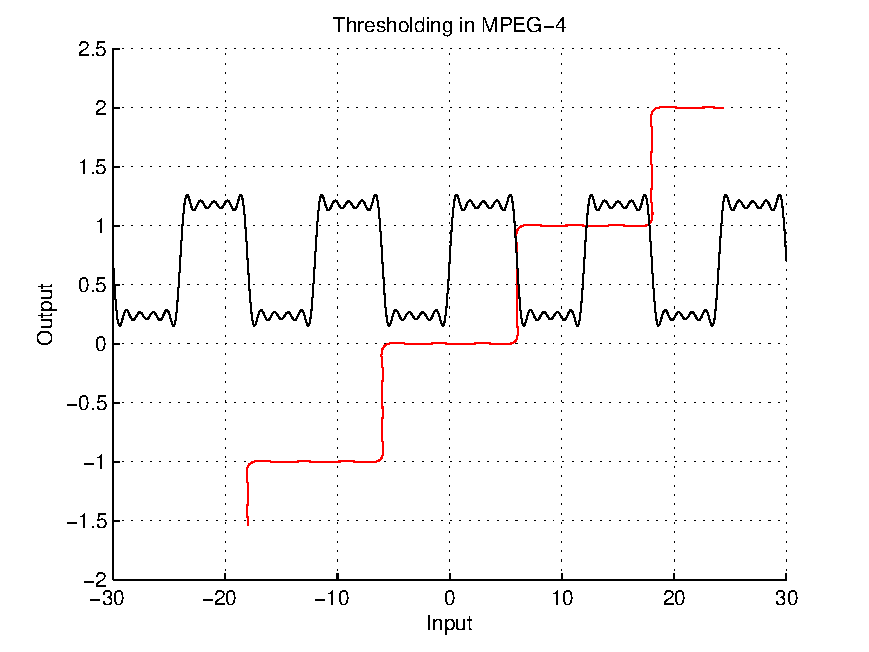
\includegraphics[width=0.45\textwidth]{figs/Quantization_8_result_plot_squareWave}
		\caption{A secondary square wave is generated to capture the non-linearities in the quantization process.  It depends on the input and $Qp$.}
		\label{fig:Square_Wave}
		\end{figure}
			
\item \textbf{Square wave 2}. The next step is to use $y$ to find $z$.  $z$ can take on two different values, $z_1$ and $z_2$, depending on the input.  In Figure~\ref{fig:Model2_b}, $z=z_1$ if $x$ is between points $A$ and $D$ and $z=z_2$ if $x$ is between points $D$ and $C$.  $z_1$ and $z_2$ are given by,  

		\begin{align}
		z_1&=0.707y_1\notag\\
		z_2&=0.707(1.414Qp)- y_2\notag\\ 
		\label{eq:Formulas_for_z}
		\end{align}	

		%figure: Fourier Series modeling
%		\begin{figure}
%		\centering				
%		\includegraphics[width=0.45\textwidth]{figs/Output.eps}
%		\caption{Continuous Time Fourier Series modeling}
%		\label{fig:Output}
%		\end{figure}

		\begin{figure}[t]
		\centering				
		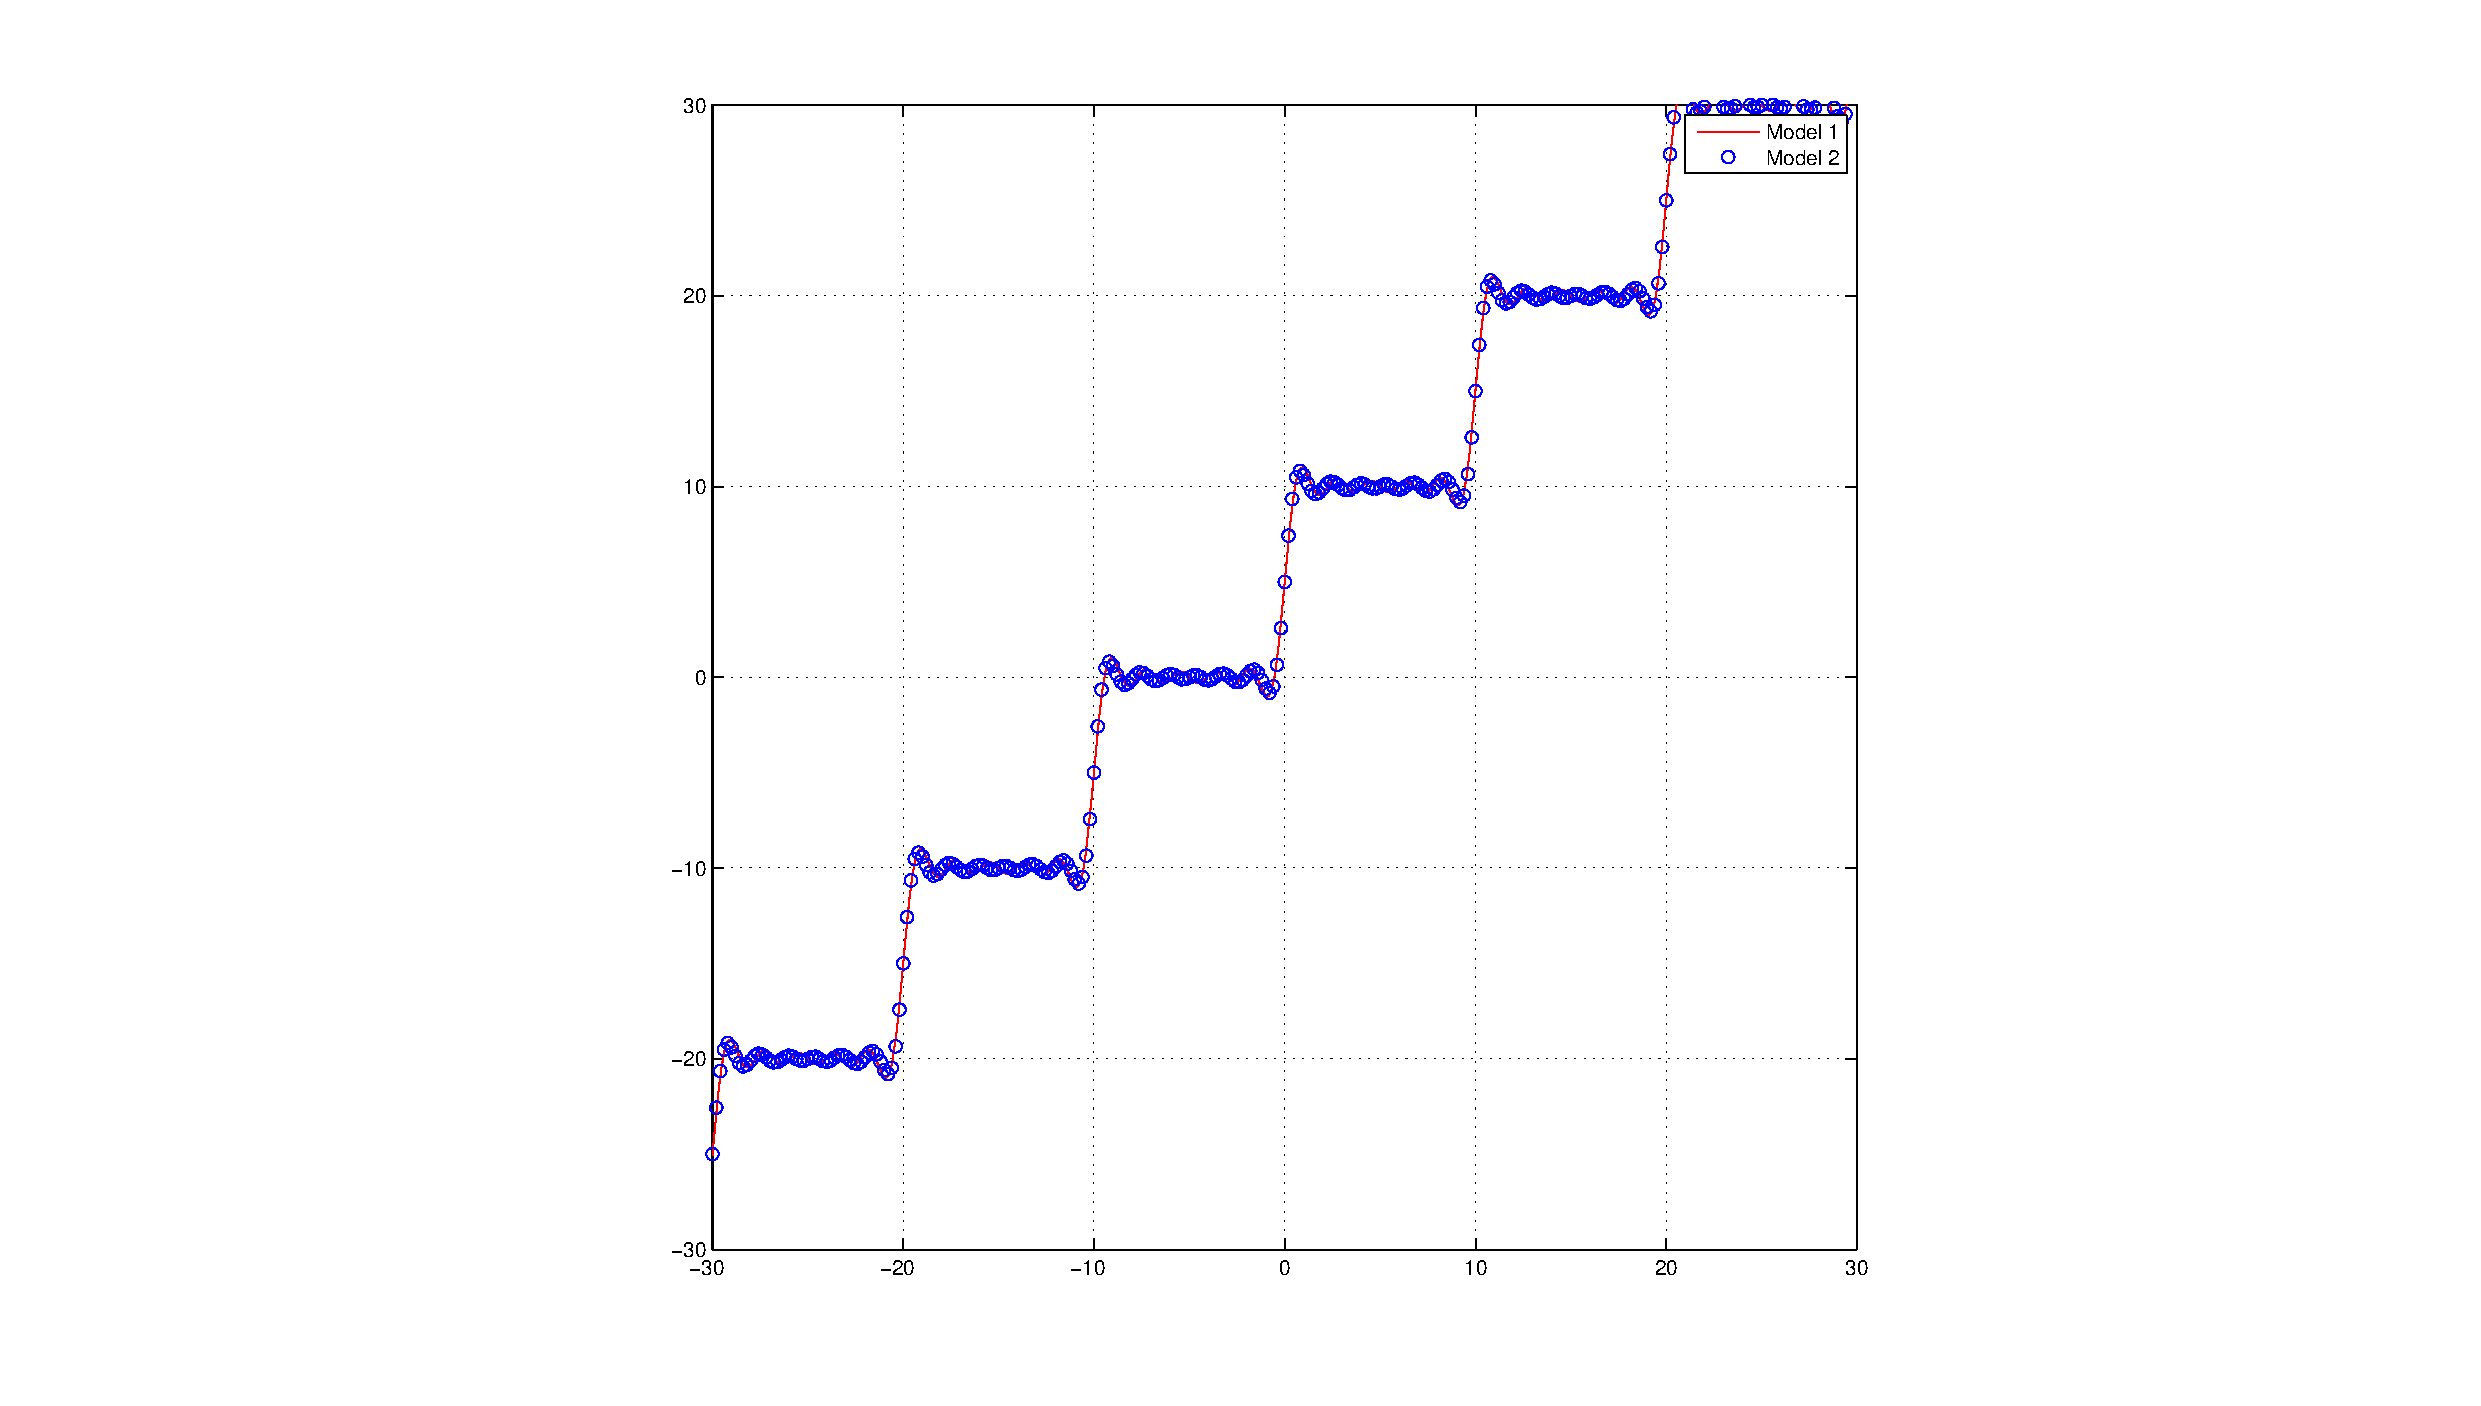
\includegraphics[width=1.0\textwidth]{figs/Quantization_9_result_finalPlot_staircase}
		\caption{Plotting analytical equations derived in Models 1 and 2.}
		\label{fig:Matlab_StaircaseFunction_Models_1_2}
		\end{figure}
				
This pattern repeats for all triangles.  The amplitude of $z$ can therefore be modeled as another square wave.  Once again we start with the square wave in Equation~\ref{eq:Square_Wave_shifted}, and using parameters, 
%$A=(0.707(1.414Qp)- y) - 0.707y = Qp-0.707y - 0.707y = Qp - 1.414y$, %$T1=\frac{Qp}{4}$, $T=Qp$, $t_0=T_1$, and $y_0=0.707y$, 

		\begin{align}
		\label{eq:Parameter_values_2}
		A			&=	(0.707(1.414Qp)- y) - 0.707y\notag\\
		  		&=	Qp-0.707y - 0.707y\notag\\
		  		&=	Qp - 1.414y\notag\\
		T1		&=	\frac{Qp}{4}\notag\\ 
		T			&=	Qp\notag\\
		w_0 	&=	\frac{2 \ \pi}{Qp}\\
		t_0		&=	T_1\notag\\
		y_0		&=	0.707 \ y \ + 2A\frac{T_1}{T}\notag\\
		   		&=	0.707 \ y + \frac{Qp}{2} - 0.707 \ y\notag\\
		   		&=	\frac{Qp}{2}
		\end{align}	

we get,

		\begin{equation}
		c_{s_2}[k] = (\frac{Qp}{2} - \frac{y}{\sqrt{2}}) \ c_{s_1}[k]
		\label{eq:Square_2_ck}
		\end{equation}
		
where, $c_{s_1}[k]$ is defined in Equation~\ref{eq:Square_1_ck}.  $z$ can now be found using,

		\begin{align}
		z[x] &= DC + 2 \ c_{s_2}[1] \ cos( w_0 \ x) + 2 \ c_{s_2}[3] \ cos(3 \ w_0 \ x) + 2 \ c_{s_2}[5] \ cos(5 \ w_0 \ x)\notag\\
		 			 &= DC + 2 \ c_{s_2}[1] \ cos( \frac{2 \ \pi}{Qp}x) + 2 \ c_{s_2}[3] \ cos(3 \ \frac{2  \  \pi}{Qp}x) + 2 \ c_{s_2}[5] \ cos(5 \ \frac{2  \ \pi}{Qp}x)
		\label{eq:Square_2_time}
		\end{align}
		
This square wave is plotted in Figure~\ref{fig:Square_Wave}.

\item As a result of all these steps, the staircase function, $x+z$ is plotted in Figure~\ref{fig:Matlab_StaircaseFunction_Models_1_2}.
\end{itemize}
		



%------------------------------------------------------------------------------------------------------------------------------
\section{CONCLUSIONS}
%------------------------------------------------------------------------------------------------------------------------------
In this paper, we develop two methods for finding an analytical expression for a staircase function.  Both are based on the Continuous Time Fourier Series.  Whereas the first is well-known, the second method is based on two successive applications of the CTFS.  The goal of presenting this alternate way of modeling the quantization function is that it may be useful in finding integral values of the quantization step size, and may also find use in a variety of applications that use quantization.

%------------------------------------------------------------------------------------------------------------------------------
%BIBLIOGRAPHY
%------------------------------------------------------------------------------------------------------------------------------

\bibliography{MyCitations}  
\end{document}
